\documentclass[10pt]{article}

\usepackage{algorithm,algpseudocode}
\usepackage{a4wide,amsmath,amssymb,fancyhdr,graphicx,tabularx,xspace}
\usepackage{tikz}
\usetikzlibrary{arrows.meta}
%------------------------------------------------------------------------------
\newcommand{\course}{}
\newcommand{\coursenumber}{}
\newcommand{\courseyear}{}
%------------------------------------------------------------------------------
\pagestyle{fancy}
\chead{}
\lhead{-}
\rhead{\course\ Text Assignment \courseyear}
\cfoot{\thepage}
\lfoot{}
\rfoot{}
%------------------------------------------------------------------------------

%to include IPE/pdf correctly
\expandafter\ifx\csname pdfoptionalwaysusepdfpagebox\endcsname\relax\else
\pdfoptionalwaysusepdfpagebox5
\fi


\newcommand{\Reals}{{\Bbb R}}
\newcommand{\Nats}{{\Bbb N}}
\newcommand{\Ints}{{\Bbb Z}}

\newcommand{\C}{\ensuremath{\mathcal{C}}}
\newcommand{\E}{\ensuremath{\mathcal{E}}}
\newcommand{\F}{\ensuremath{\mathcal{F}}}
\newcommand{\G}{\ensuremath{\mathcal{G}}}
\newcommand{\U}{\ensuremath{\mathcal{U}}}

\newcommand{\graph}{\ensuremath{\mathcal{G}}}
\newcommand{\tree}{\ensuremath{\mathcal{T}}}
\newcommand{\node}{\nu}
\newcommand{\lchild}{\mathrm{lc}}
\newcommand{\rchild}{\mathrm{rc}}
\newcommand{\size}{\mathit{size}}
\newcommand{\leaf}{\mu}
\newcommand{\mylist}{{\cal L}}
\newcommand{\myroot}{\mathit{root}}
\newcommand{\key}{\mathit{key}}
\newcommand{\bd}{\partial}

\newcommand{\myopt}{\mbox{{\sc opt}}\xspace}
\newcommand{\lb}{\mbox{{\sc lb}}\xspace}
\newcommand{\loadb}{{\sc Load Balancing}\xspace}

\newcommand{\vc}{{\sc Vertex Cover}\xspace}
\newcommand{\wvc}{{\sc Weighted Vertex Cover}\xspace}
\newcommand{\wsetc}{{\sc Weighted Set Cover}\xspace}
\newcommand{\tsp}{{\sc TSP}\xspace}
\newcommand{\mst}{{\sc MST}\xspace}

\newcommand{\eps}{\varepsilon}
\newcommand{\ol}{\overline}
\renewcommand{\leq}{\leqslant}
\renewcommand{\geq}{\geqslant}

\newcommand{\pr}[1]{\Pr[#1]}
\DeclareMathOperator{\expectation}{E}
\newcommand{\expt}[1]{\expectation[#1]}
\newcommand{\events}[1]{\mbox{Events}(#1)}
\newcommand{\rank}{\mathit{rank}}
\newcommand{\result}{\mathit{result}}
\newcommand{\piv}{\mathrm{piv}}
\newcommand{\myexp}{\mathrm{exp}}
\newcommand{\best}{\mathrm{best}}
\newcommand{\worst}{\mathrm{worst}}
\newcommand{\dest}{\mathit{dest}}
\newcommand{\dist}{\mathit{distance}}
\newcommand{\weight}{\mathit{weight}}
\newcommand{\mylength}{\mathit{length}}
\newcommand{\length}{\mathit{length}}
\newcommand{\alg}{{\sc Alg}\xspace}

\newcommand{\start}{\mathit{start}}
\newcommand{\myend}{\mathit{end}}
\newcommand{\free}{\mathit{free}}
\newcommand{\true}{{\sc True}\xspace}
\newcommand{\false}{{\sc False}\xspace}

\newcommand{\etal}{{\emph{et al.}\xspace}}


%------------------------------------------------------------------------------
% Theorem-Like Environments
%------------------------------------------------------------------------------
\newtheorem{defin}{Definition}
\newenvironment{mydefinition}{\begin{defin} \sl}{\end{defin}}
\newtheorem{theo}[defin]{Theorem}
\newenvironment{mytheorem}{\begin{theo} \sl}{\end{theo}}
\newtheorem{lem}[defin]{Lemma}
\newenvironment{mylemma}{\begin{lem} \sl}{\end{lem}}
\newtheorem{propo}[defin]{Proposition}
\newenvironment{myproposition}{\begin{propo} \sl}{\end{propo}}
\newtheorem{coro}[defin]{Corollary}
\newenvironment{corollary}{\begin{coro} \sl}{\end{coro}}

\newenvironment{myproof}{\emph{Proof.}}{\hfill $\Box$ \medskip\\}

%------------------------------------------------------------------------------
\newcounter{rcounter}
\newenvironment{rlist}%
{\begin{list}{\setnr-\arabic{rcounter}}{\usecounter{rcounter}}}{\end{list}}
\newcounter{rcountermem}
%------------------------------------------------------------------------------

\title{Solutions}
\author{Natasja van de L'Isle - 1022588}
\date{18/02/2016}


\begin{document}
	
	
	%------------------------------------------------------------------------------
	\newcommand{\setnr}{Exercise}
	\subsection*{Exercises}
	%------------------------------------------------------------------------------
	\begin{rlist}
\item

\begin{figure}
\centering
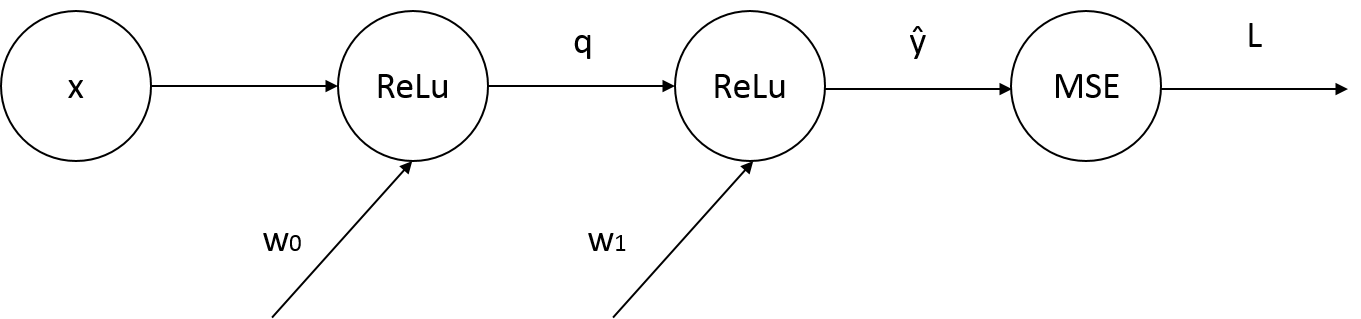
\includegraphics[width=0.75\textwidth]{Q1_graph}
\caption{Graph}
\end{figure}

We can use two approaches to compute new values for the weights $w_0$ and $w_1$. The first one is to update the weights after each observation. The second is to take the average of the computed weights and thus, only update once.

Observations: $(x_1,y_1) = (1,2)$ and $(x_2,y_2) = (2,3)$
Weights: $w_0 = 1$ and $w_1 = 2$

We use the MSE as loss function: $L = \frac{1}{2} (\hat{y}-y)^2$

%$L = \frac{1}{2n}\sum_{i=0}^n(\hat{y}_i-y_i)^2$

\begin{enumerate}
\item Approach one:

$\hat{y}_1 = w_1(w_0x_1) = 2*1*1 = 2$

$L = \frac{1}{2}(2-2)^2 = 0$

As $L=0$ the derivatives will all be zero and, therefore, the weights will not be updated. Thus, we continue to the next observation.

$\hat{y}_2 = w_1(w_0x_2) = 2*1*2 = 4$

$L = \frac{1}{2}(4-3)^2 = \frac{1}{2}$

\begin{align*}
\frac{\partial L}{\partial \hat{y_2}} &= [\frac{1}{2} (\hat{y_2}-y_2)^2]'\\
	&= 2*\frac{1}{2} (\hat{y_2}-y_2) * 1\\
	&= \hat{y_2}-y_2 \\
	&= 1\\
\end{align*}

\begin{align*}
\frac{\partial L}{\partial w_1} &= \frac{\partial \hat{y_2}}{\partial w_1} \frac{\partial L}{\partial \hat{y_2}}\\
	&=  w_0x_2*\frac{\partial L}{\partial \hat{y_2}}\\
	&=  2*\frac{1}{2}\\
	&= 1\\
\end{align*}

\begin{align*}
\frac{\partial L}{\partial q} &= \frac{\partial \hat{y_2}}{\partial q} \frac{\partial L}{\partial \hat{y_2}}\\
	&= w_1 * 1\\
	&= 2
\end{align*}

\begin{align*}
\frac{\partial L}{\partial w_0} &= \frac{\partial q}{\partial w_0} \frac{\partial L}{\partial q}\\
	&= x_2 *\frac{\partial L}{\partial q}\\
	&= 2*2 = 4
\end{align*}



Thus, $w_1^* = w_1-0.1*2 = 1.8$ and $w_0^* = w_0 - 0.1*4 = 0.6$.

\item Approach two:
\end{enumerate}
	\end{rlist}

\end{document}